\documentclass[tikz, border=10pt]{standalone}
\usepackage{pgfplots}
\usepgfplotslibrary{groupplots}
\pgfplotsset{compat=1.18}

\begin{document}
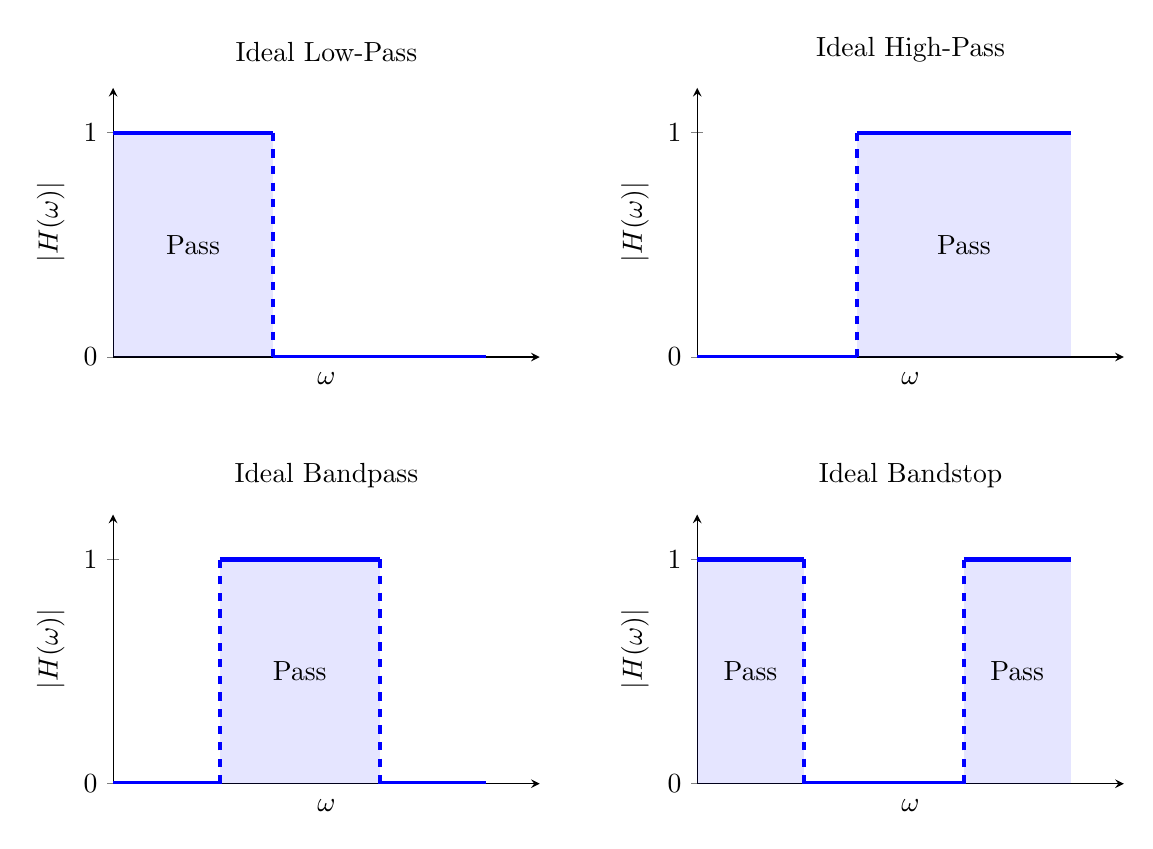
\begin{tikzpicture}
    \begin{groupplot}[
        group style={
            group size=2 by 2,
            vertical sep=2cm,
            horizontal sep=2cm,
        },
        width=7cm, height=5cm,
        xmin=0, xmax=4,
        ymin=0, ymax=1.2,
        grid=none,
        axis lines=left,
        xtick=\empty,
        ytick={0, 1},
        yticklabels={0, 1},
        xlabel={$\omega$},
        ylabel={$|H(\omega)|$},
    ]

    % Low-Pass Filter
    \nextgroupplot[title={Ideal Low-Pass}]
    \draw[ultra thick, blue] (axis cs: 0, 1) -- (axis cs: 1.5, 1);
    \draw[ultra thick, blue, dashed] (axis cs: 1.5, 1) -- (axis cs: 1.5, 0);
    \draw[ultra thick, blue] (axis cs: 1.5, 0) -- (axis cs: 3.5, 0);
    \node[below] at (axis cs: 1.5, 0) {$\omega_c$};
    \fill[blue, opacity=0.1] (axis cs: 0, 0) rectangle (axis cs: 1.5, 1);
    \node at (axis cs: 0.75, 0.5) {Pass};

    % High-Pass Filter
    \nextgroupplot[title={Ideal High-Pass}]
    \draw[ultra thick, blue] (axis cs: 0, 0) -- (axis cs: 1.5, 0);
    \draw[ultra thick, blue, dashed] (axis cs: 1.5, 0) -- (axis cs: 1.5, 1);
    \draw[ultra thick, blue] (axis cs: 1.5, 1) -- (axis cs: 3.5, 1);
    \node[below] at (axis cs: 1.5, 0) {$\omega_c$};
    \fill[blue, opacity=0.1] (axis cs: 1.5, 0) rectangle (axis cs: 3.5, 1);
    \node at (axis cs: 2.5, 0.5) {Pass};

    % Bandpass Filter
    \nextgroupplot[title={Ideal Bandpass}]
    \draw[ultra thick, blue] (axis cs: 0, 0) -- (axis cs: 1, 0);
    \draw[ultra thick, blue, dashed] (axis cs: 1, 0) -- (axis cs: 1, 1);
    \draw[ultra thick, blue] (axis cs: 1, 1) -- (axis cs: 2.5, 1);
    \draw[ultra thick, blue, dashed] (axis cs: 2.5, 1) -- (axis cs: 2.5, 0);
    \draw[ultra thick, blue] (axis cs: 2.5, 0) -- (axis cs: 3.5, 0);
    \node[below] at (axis cs: 1, 0) {$\omega_1$};
    \node[below] at (axis cs: 2.5, 0) {$\omega_2$};
    \fill[blue, opacity=0.1] (axis cs: 1, 0) rectangle (axis cs: 2.5, 1);
    \node at (axis cs: 1.75, 0.5) {Pass};

    % Bandstop Filter
    \nextgroupplot[title={Ideal Bandstop}]
    \draw[ultra thick, blue] (axis cs: 0, 1) -- (axis cs: 1, 1);
    \draw[ultra thick, blue, dashed] (axis cs: 1, 1) -- (axis cs: 1, 0);
    \draw[ultra thick, blue] (axis cs: 1, 0) -- (axis cs: 2.5, 0);
    \draw[ultra thick, blue, dashed] (axis cs: 2.5, 0) -- (axis cs: 2.5, 1);
    \draw[ultra thick, blue] (axis cs: 2.5, 1) -- (axis cs: 3.5, 1);
    \node[below] at (axis cs: 1, 0) {$\omega_1$};
    \node[below] at (axis cs: 2.5, 0) {$\omega_2$};
    \fill[blue, opacity=0.1] (axis cs: 0, 0) rectangle (axis cs: 1, 1);
    \fill[blue, opacity=0.1] (axis cs: 2.5, 0) rectangle (axis cs: 3.5, 1);
    \node at (axis cs: 0.5, 0.5) {Pass};
    \node at (axis cs: 3, 0.5) {Pass};

    \end{groupplot}
\end{tikzpicture}
\end{document}
